%Bendri panaudojamumo vertinimo klausimynai:
%\begin{itemize}
  %\item SUMI (Software Usability Measurement Inventory)
  %\item QUIS (Questionnaire for User Interaction Satisfaction)
%\end{itemize}
%Parengti savybių sąrašą (konspekto 96 psl.)


%Vertinimo kriterijai testuojant:
%\begin{itemize}
  %\item kiek kartų teko grįžti į pagrindinį meniu be reikalo;
  %\item kiek kartų buvo užuominų ar paraginimų;
  %\item kiek kartų buvo atverstas puslapis nurodantis puslapio žemėlapį
    %(struktūrą);
  %\item abejojimų skaičius (ir jų trukmė);
  %\item užduotys, kurios neatitinka sėkmės kriterijaus;
  %\item klaidų aprašas ir sunkumų nustatymas;
  %\item klaidų priežasčių nustatymas;
%\end{itemize}

\subsection{Testuojamos užduotys}

Testavimo metu buvo tikrinama, kaip sistemos naudotojai atlieka
užduotis „Apkrovų skaičiavimas“ ir „Laisviausių laiko
intervalų paieška“. Užduočių formuluotės pateiktos
\ref{fig:uzduotis_1} ir \ref{fig:uzduotis_2} paveikslėliuose.
Testuojant buvo siekiama išmatuoti kiek reikia laiko įvykdyti
kiekvienai užduoties daliai bei dalies vykdymo sudėtingumą pagal tai
keliems testuotojams pavyko visiškai sėkmingai atlikti tą dalį.
Laikoma, kad testuojantysis visiškai sėkmingai įvykdė užduotį dalį,
jei:
\begin{itemize}
  \item pasinaudodamas sistema gavo teisingus rezultatus;
  \item nė karto nesikreipė pagalbos į asistentą.
\end{itemize}

TODO: Surašyti sėkmės matus. Reikėtų remtis tuo kas buvo surašyta
„Panaudojamumo tiksluose“ 2 ŽKS darbe, bet tai nebūtinai turi būti
kopijavimas iš ten, nes mes dabar žinom daugiau informacijos.

TODO: Kriterijai: užduoties dalies įvykdymo laikas (sėkmės matai iš
tikslų) ir ar įvykdė užduotį.

\begin{figure}[H]
  \begin{center}
    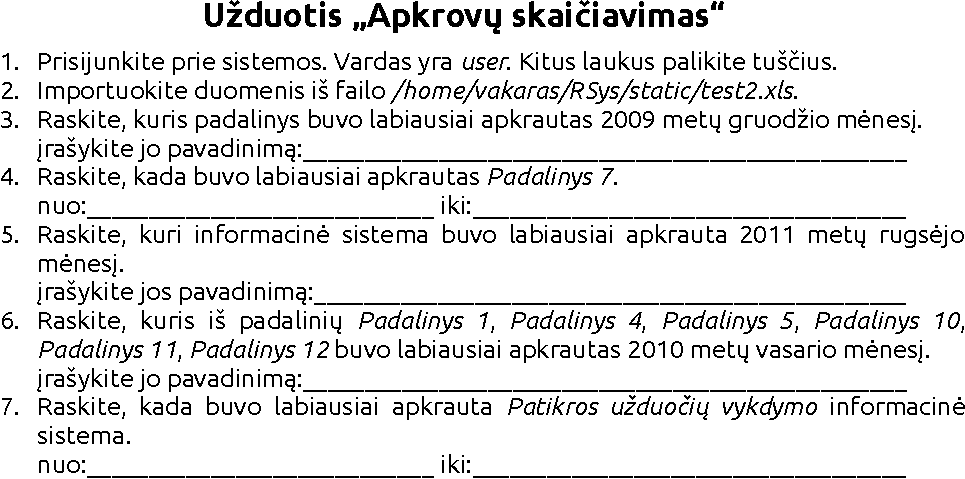
\includegraphics[width=0.9\textwidth]{./4/pdfs/uzduotis1.pdf}
  \end{center}
  \caption{Pirma užduotis}
  \label{fig:uzduotis_1}
\end{figure}

\begin{figure}[H]
  \begin{center}
    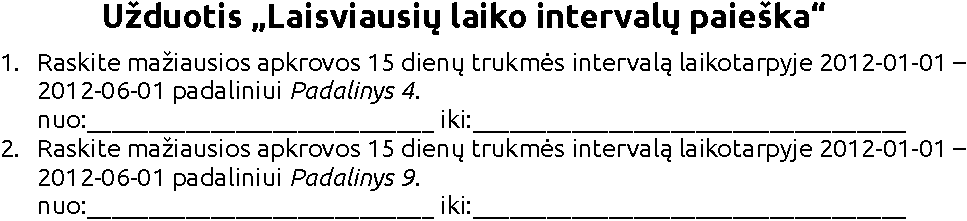
\includegraphics[width=0.9\textwidth]{./4/pdfs/uzduotis2.pdf}
  \end{center}
  \caption{Antra užduotis}
  \label{fig:uzduotis_2}
\end{figure}

\subsection{Metodas}

Testavimo vykdymo eiga:
\begin{enumerate}
  \item testuojantysis pasirašo sutikimą;
  \item testuojantysis užpildo klausimyną apie jo patirtį;
  \item testuojančiajam duodama užduotis ir jis ją bando atlikti
    pasinaudodamas programa, garsiai komentuodamas ką bando daryti;
    vykdytojas tuo metu sėdi šalia, žymisi pastabas bei per kiek
    laiko testuojantysis įvykdė užduoties dalį (galimas ir nuotolinis
    būdas, kai testuotojas pats žymi pastabas ir laikus);
  \item testuojantysis užpildo klausimyną apie naudojimosi programa
    įspūdžius.
\end{enumerate}

% Mano gauti atsakymai:
% \begin{verbatim}
% 3: „Padalinys 1“
% 4: 2008-05 (10245,5), 2010-03 (10152,5), 2010-05 (10137), 2011-06 (10290) – norimas atsakymas: 2011-06-01 – 2011-07-01;
% 5: IS1, Finansų apskaitos ir valdymo;
% 6: „Padalinys 12“;
% 7: 2009-04 (35295), 2010-03 (35913,5), 2011-05 (34999) – norimas atsakymas: 2010-03-01 – 2010-04-01;
% 1: 2012-02-13 – 2012-02-28;
% 2: 2012-02-18 – 2012-03-04;
% \end{verbatim}

\subsection{Aplinka}

Keturi žmonės sistemą testavo kavinėje: vienas sėdi su vykdytoju
prie kompiuterio, kiti tuo tarpu sėdi netoliese ir šnekasi apie
pašalinius dalykus. Vienas žmogus testavo sistemą namie, visą
reikiamą įrangą įsirašęs į savo kompiuterį. Testavimo metu buvo
naudojama šviežiai įdiegta Ubuntu 11.10 operacinė sistema su Unity
grafine aplinka.

\subsection{Dalyviai}

Visi dalyviai yra skirtingų profesijų atstovai, atitinkantys
„Naudotojų kvalifikaciniai reikalavimai“ skyrelyje aprašytus reikalavimus
vadovams ir asistentui. 4 iš 5 dalyvių su dalykine sritimi ir kuriamos
sistemos paskirtimi buvo trumpai supažindinti prieš testavimą, o
penktasis tai žinojo jau iš anksčiau. Visi testuotojai buvo jauni žmonės,
19 – 30 metų amžiaus, turintys didesnę nei 3 metų darbo su skaičiuoklėmis
ir rašyklėmis patirtį. Detalesnė informacija apie kiekvieną testuotoją
pateikta lentelėse:

\xtable
{
  w [ 1 | 1 | 1 | 1 | 1 ]
  a [ p | p | p | p | p ]
  h [
    Testuotojas |
    Užimamos pareigos |
    Lytis |
    Naudojasi Ubuntu |
    Naudojasi Windows
    ]
  %
  e [ A | Projektų vadovė | Moteris | Taip | Taip ]
  e [ B | Inžinierius | Vyras | Taip | Taip ]
  e [ C | Administratorius (savanoris) | Vyras | Ne | Taip ]
  e [ D | Administratorė (savanorė) | Moteris | Ne | Taip ]
  e [ E | Programų sistemų studentė | Moteris | Taip | Taip ]
}

\xtable
{
  w [ 1 | 2 | 2 ]
  a [ p | p | p ]
  h [
    Testuotojas |
    Prie kompiuterio būna namie |
    Prie kompiuterio būna darbe
    ]
  %
  e [ A | $< 1$ valandas | $> 8$ valandas ]
  e [ B | $< 1$ valandas | $> 8$ valandas ]
  e [ C | 3–8 valandas   | 3–8 valandas   ]
  e [ D | 1–3 valandas   | 1–3 valandas   ]
  e [ E | 3–8 valandas   | 1–3 valandas   ]
}
